\documentclass[tikz]{standalone}
\usepackage{tikz}
\usetikzlibrary{positioning, graphs}
\usetikzlibrary{graphs.standard}
\begin{document}
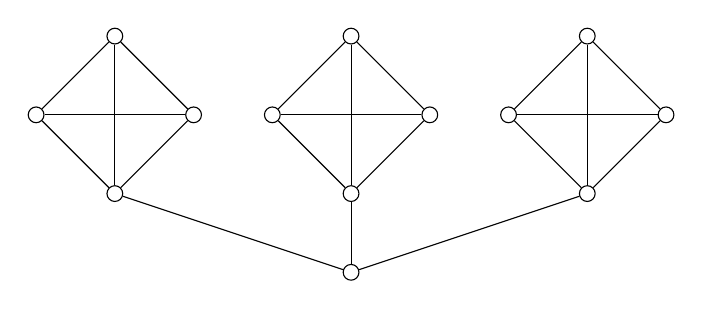
\begin{tikzpicture}
		[vertex/.style={draw,circle,inner sep = 0mm, minimum size = 2mm},
		 edgelabel/.style = {fill = white, inner sep = 0mm, font=\tiny}]
		\node[vertex] at (0,0)	(a 0) {};
		\node[vertex] at (1,1)	(a 1) {};
		\node[vertex] at (1,-1)	(a 2) {};
		\node[vertex] at (2,0)	(a 3) {};
		\node[vertex] at (3,0)	(b 0) {};
		\node[vertex] at (4,1)	(b 1) {};
		\node[vertex] at (4,-1)	(b 2) {};
		\node[vertex] at (5,0)	(b 3) {};
		\node[vertex] at (6,0)	(c 0) {};
		\node[vertex] at (7,1)	(c 1) {};
		\node[vertex] at (7,-1)	(c 2) {};
		\node[vertex] at (8,0)	(c 3) {};
		\node[vertex] at (4,-2)	(P) {};
		
		\foreach \i [evaluate={\j=int(mod(\i+1,4));}] in {0, 1, 2, 3}{
			\draw (a \i) -- (a \j);
			\draw (b \i) -- (b \j);
			\draw (c \i) -- (c \j);
		}
		\foreach \i [evaluate={\j=int(\i+2);}] in {0, 1}{
			\draw (a \i) -- (a \j);
			\draw (b \i) -- (b \j);
			\draw (c \i) -- (c \j);	
		}
		\draw (P) -- (a 2);
		\draw (P) -- (b 2);
		\draw (P) -- (c 2);
\end{tikzpicture}
\end{document}